\documentclass{beamer}

% for themes, etc.
\mode<presentation>
%\usetheme{Warsaw}
%\usecolortheme{dolphin}
%{\usetheme{Singapore}}
%{ \usetheme{lined} }
{\usetheme{Dresden}}
\usepackage{fontspec}   %加這個就可以設定字體
\usepackage{xeCJK}       %讓中英文字體分開設置
\setCJKmainfont{標楷體} %設定中文為系統上的字型,而英文不去更動,使用原TeX字型
\XeTeXlinebreaklocale "zh"             %這兩行一定要加,中文才能自動換行
\XeTeXlinebreakskip = 0pt plus 1pt     %這兩行一定要加,中文才能自動換行
\usepackage{enumerate}%列點序號
\usepackage{amsmath,amssymb,amsfonts,booktabs}
\usepackage{epic}
\usepackage{mathpazo}  % fonts are up to you
%\usepackage{astats,epsfig}
\usepackage{graphicx,epsfig,subfigure}
\usepackage{pdftexcmds}
\usepackage{xcolor}
\usepackage{float}
\usepackage{url} %超連結
\def\UrlFont{\tt}

\newtheorem*{remark}{Remark}
\setlength{\parindent}{0mm}%第一段不縮排
\setlength{\parskip}{10pt}  % 每段間隔

\newtheorem{thm}{\bf{Theorem.}}
\renewcommand{\proofname}{\ctxfk \textbf{Proof.}}
%\usepackage{array,booktabs}
% these will be used later in the title page
\title{Convolutional Neural Networks}
\author{Yi-Ting Tsai}
\institute{National Sun Yat-sen University}
\date{2018/10/24}
\begin{document}
		\begin{frame}
		\titlepage
        \end{frame}

        \begin{frame}
		\frametitle{Outline} % make a frame titled "Outline"
		\tableofcontents % show TOC and highlight current section
        \end{frame}
\section{Review-example}
    \begin{frame}
    \frametitle{Why CNN for Image: }
        \begin{itemize}
            \item[.] Some patterns are much smaller than the whole image
            \item[.] The same patterns appear in different regions.
            \item[.] Subsampling the pixels will not change the object
        \end{itemize}
    \end{frame}

    \begin{frame}
    \frametitle{Example: }
        \begin{figure}[H]
            \begin{center}
                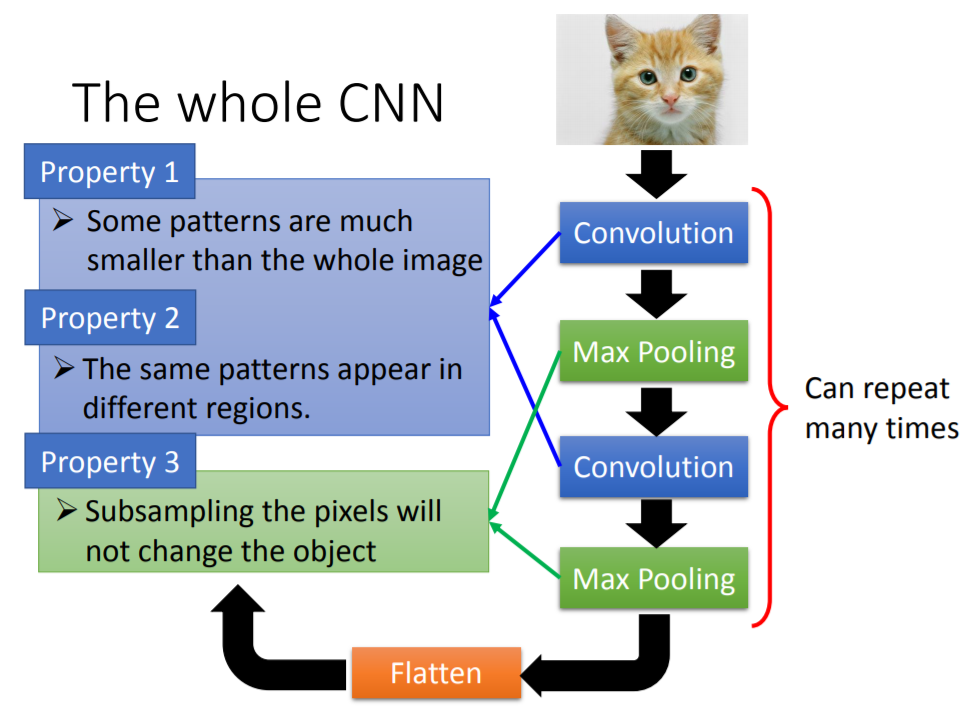
\includegraphics[width=7.5cm]{ppt1}
            \end{center}
        \end{figure}
    \end{frame}

    \begin{frame}
    \frametitle{Example: }
        \begin{figure}[H]
            \begin{center}
                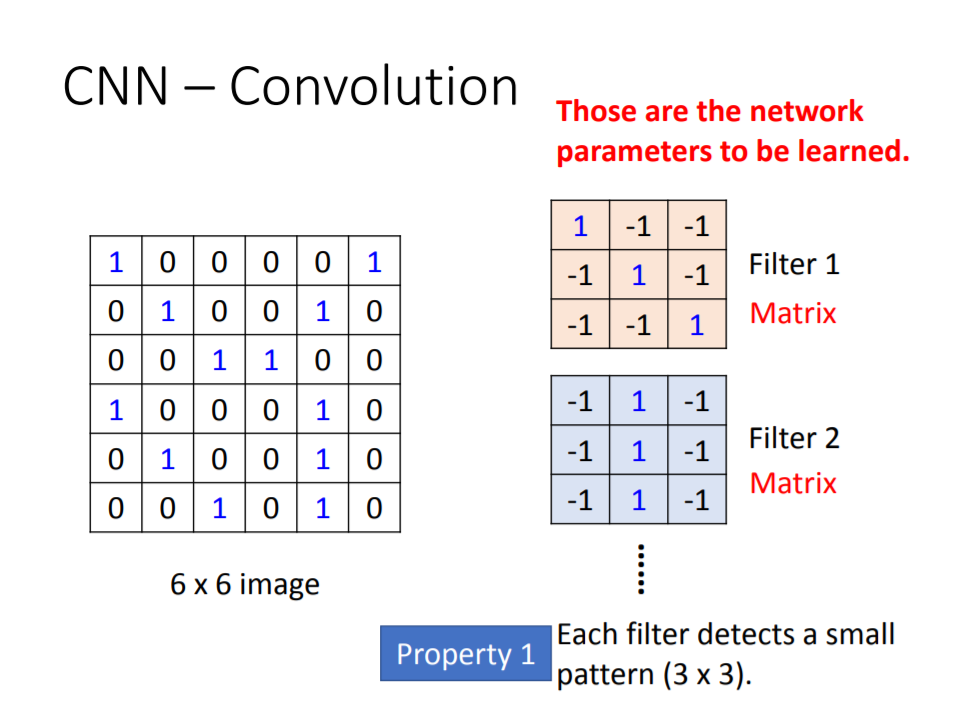
\includegraphics[width=7.5cm]{ppt2}
            \end{center}
        \end{figure}
    \end{frame}
    \begin{frame}
    \frametitle{Example: }
        \begin{figure}[H]
            \begin{center}
                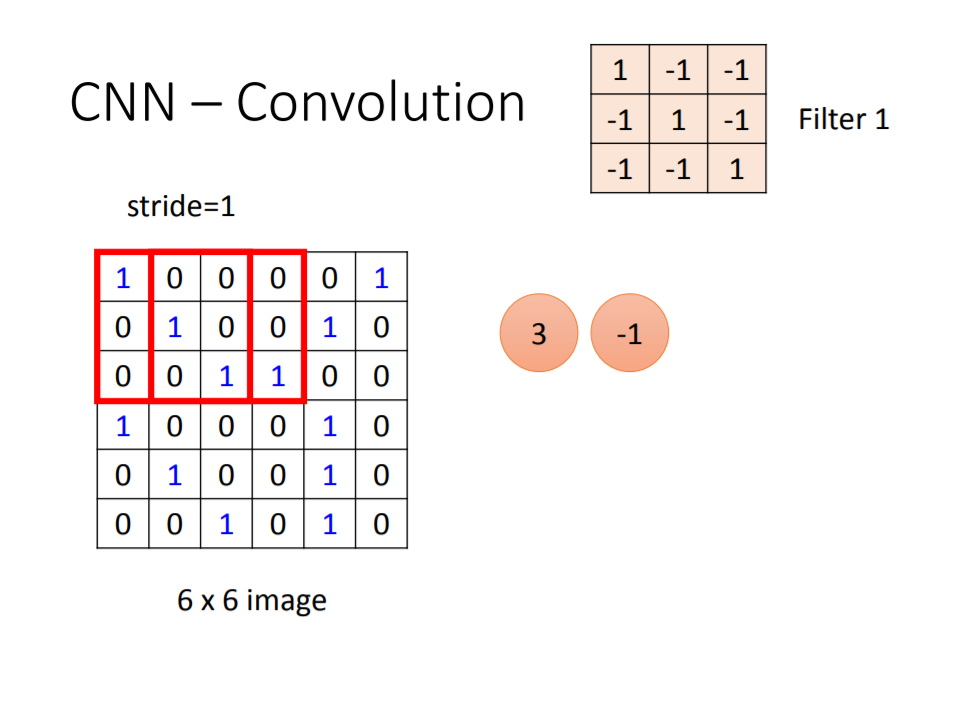
\includegraphics[width=7.5cm]{ppt3}
            \end{center}
        \end{figure}
    \end{frame}
    \begin{frame}
    \frametitle{Example: }
        \begin{figure}[H]
            \begin{center}
                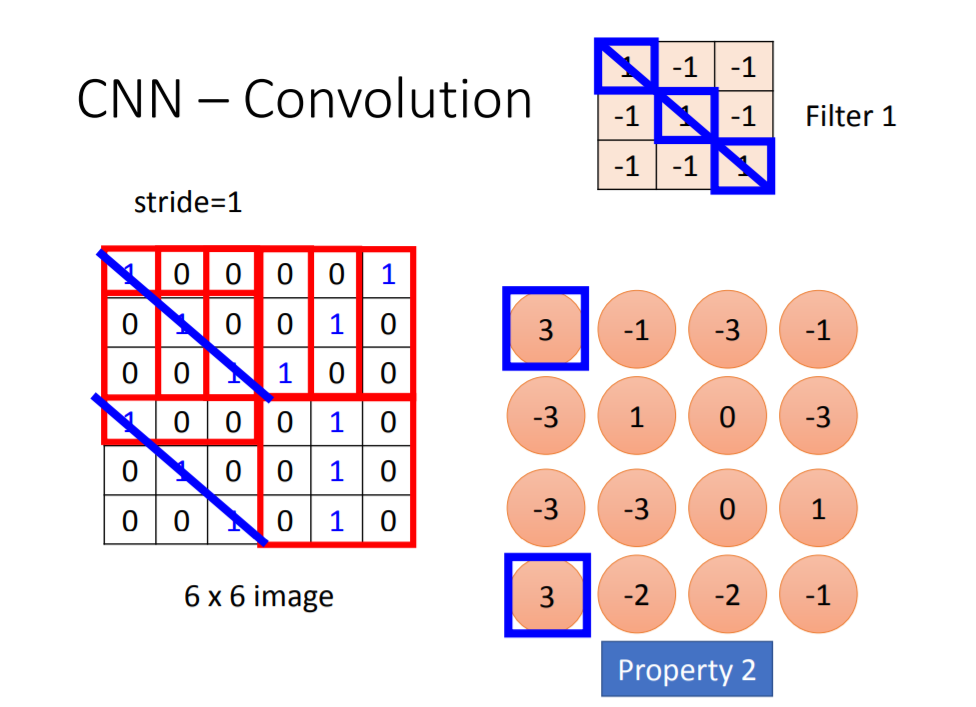
\includegraphics[width=7.5cm]{ppt4}
            \end{center}
        \end{figure}
    \end{frame}
    \begin{frame}
    \frametitle{Example: }
        \begin{figure}[H]
            \begin{center}
                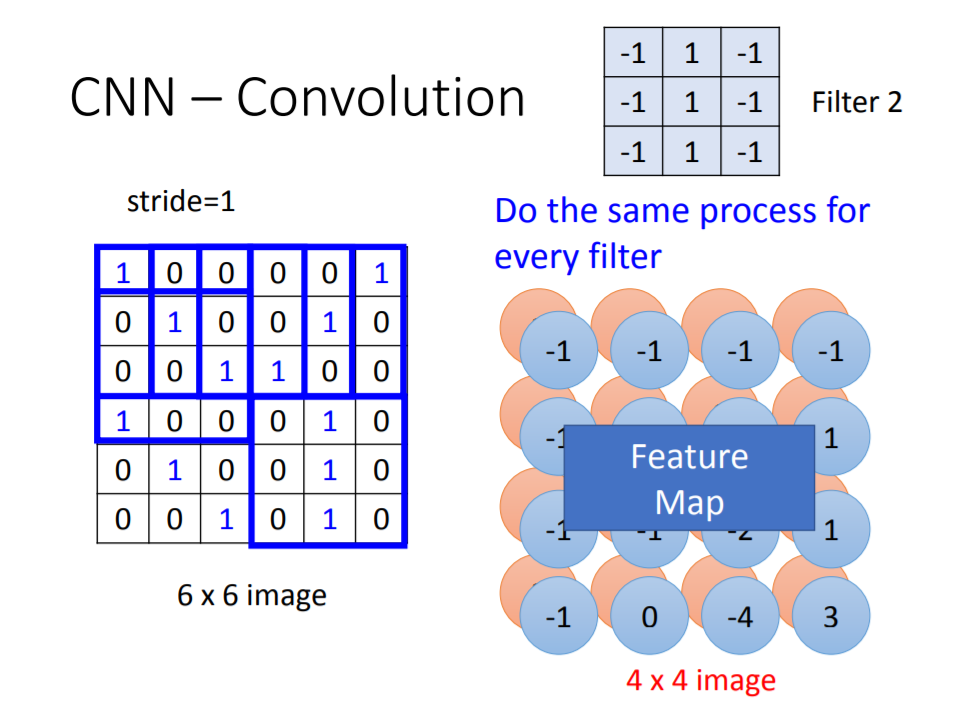
\includegraphics[width=7.5cm]{ppt5}
            \end{center}
        \end{figure}
    \end{frame}
    \begin{frame}
    \frametitle{Example: }
        \begin{figure}[H]
            \begin{center}
                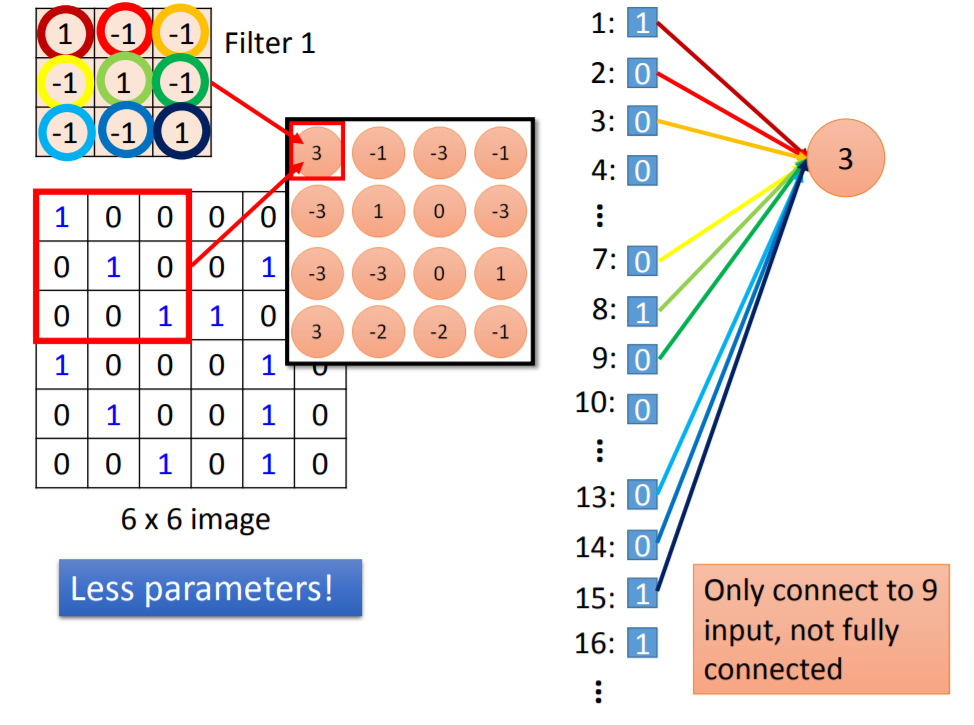
\includegraphics[width=7.5cm]{ppt6}
            \end{center}
        \end{figure}
    \end{frame}
    \begin{frame}
    \frametitle{Example: }
        \begin{figure}[H]
            \begin{center}
                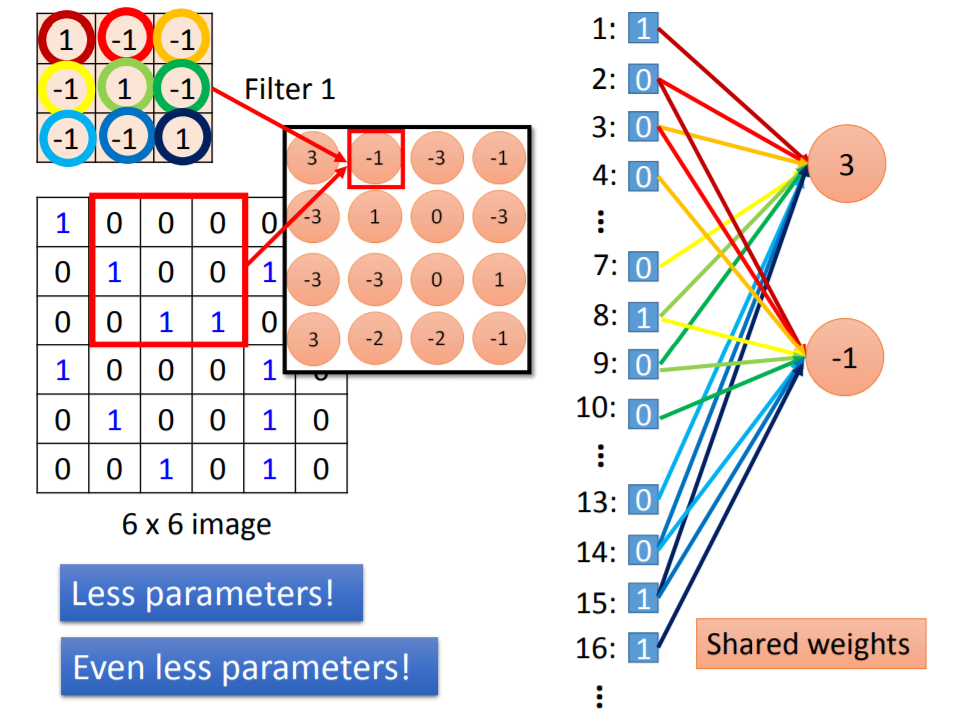
\includegraphics[width=7.5cm]{ppt7}
            \end{center}
        \end{figure}
    \end{frame}
    \begin{frame}
    \frametitle{Example: }
        \begin{figure}[H]
            \begin{center}
                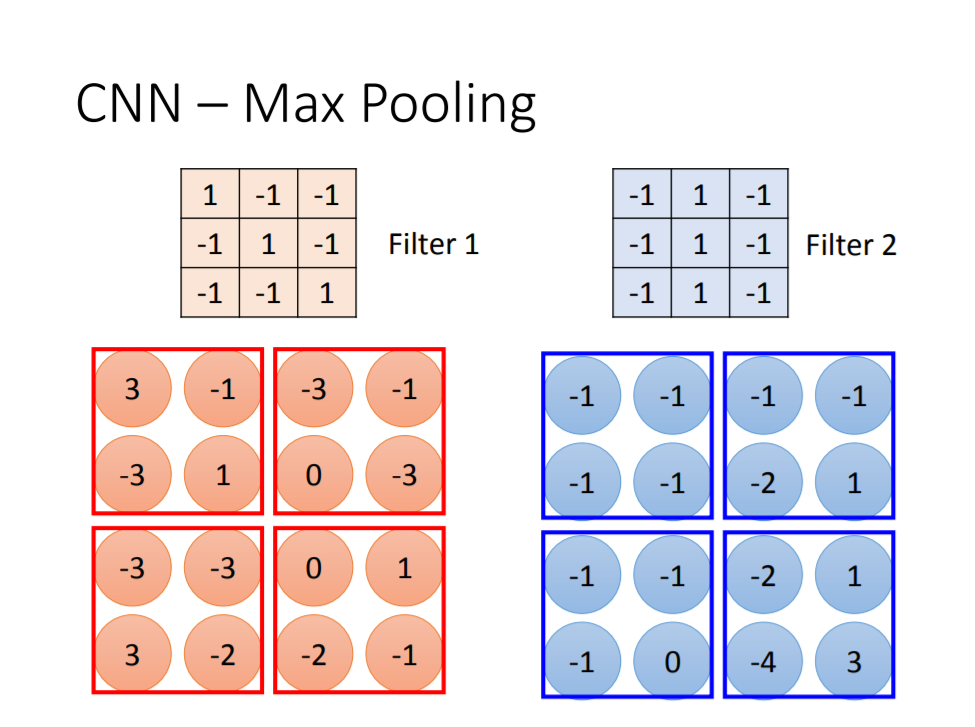
\includegraphics[width=7.5cm]{ppt8}
            \end{center}
        \end{figure}
    \end{frame}
    \begin{frame}
    \frametitle{Example: }
        \begin{figure}[H]
            \begin{center}
                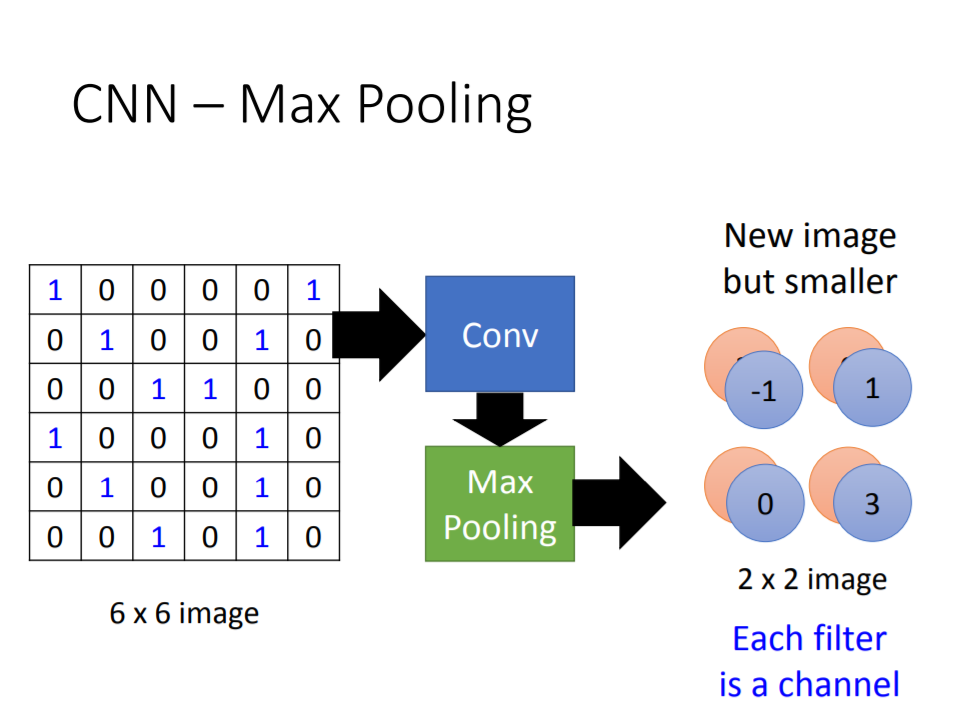
\includegraphics[width=7.5cm]{ppt9}
            \end{center}
        \end{figure}
    \end{frame}
    \begin{frame}
    \frametitle{Correction p359: }
    The sentence at the bottom of page 361 should be:

    Specifically, a neuron located in row i, column j of the feature map k in a given convolutional layer l is connected to the outputs of the neurons in the previous layer l - 1, located in rows i x sh to i x sh + fh - 1 and columns j x sw to j x sw + fw - 1, across all feature maps (in layer l - 1).
    \end{frame}
    \begin{frame}
    \frametitle{Correction p360: }
    The Equation 13-1 should be (using latexmath):
    \begin{align}
    z_{i,j,k} = b_k + \sum\limits_{u = 0}^{f_h - 1} \, \, \sum\limits_{v = 0}^{f_w - 1} \, \, \sum\limits_{k' = 0}^{f_{n'} - 1} \, \, x_{i', j', k'} . w_{u, v, k', k}
    \quad \text{with }
    \begin{cases}
        i' = i \times s_h + u \\
        j' = j \times s_w + v
    \end{cases}
    \end{align}
    \end{frame}
\section{CNN Architectures}
    \begin{frame}
    \frametitle{Typical CNN architectures: }
        \begin{figure}[H]
            \begin{center}
                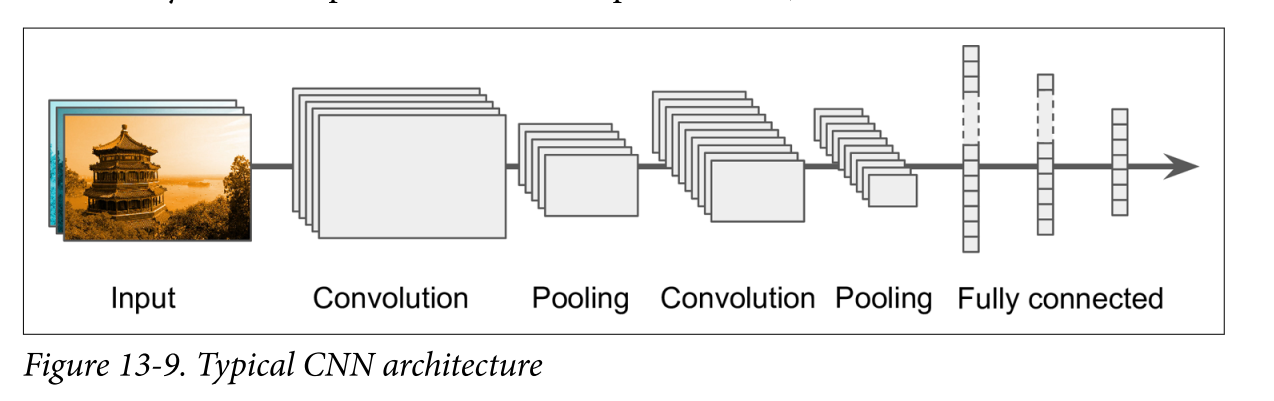
\includegraphics[width=7cm]{FIGURE13-9}
            \end{center}
        \caption{Typical CNN architecture}
        \end{figure}
    \end{frame}

    \begin{frame}
    \frametitle{CNN Architectures: }
        \par A good measure of this progress is the error rate in  competitions  such  as  the ILSVRC  ImageNet  challenge.
             In  this  competition  the top-5 error rate for image
             classification fell from over $0.26$ to barely over $0.03$ in just five years.
        \par We will first look at the classical LeNet-5 architecture (1998), then three of the winners
             of  the  ILSVRC  challenge:  AlexNet  (2012),  GoogLeNet  (2014),  ResNet(2015) , and SENet(2017) .
    \end{frame}

    \begin{frame}
    \frametitle{CNN Architectures: }
        \begin{figure}[H]
            \begin{center}
                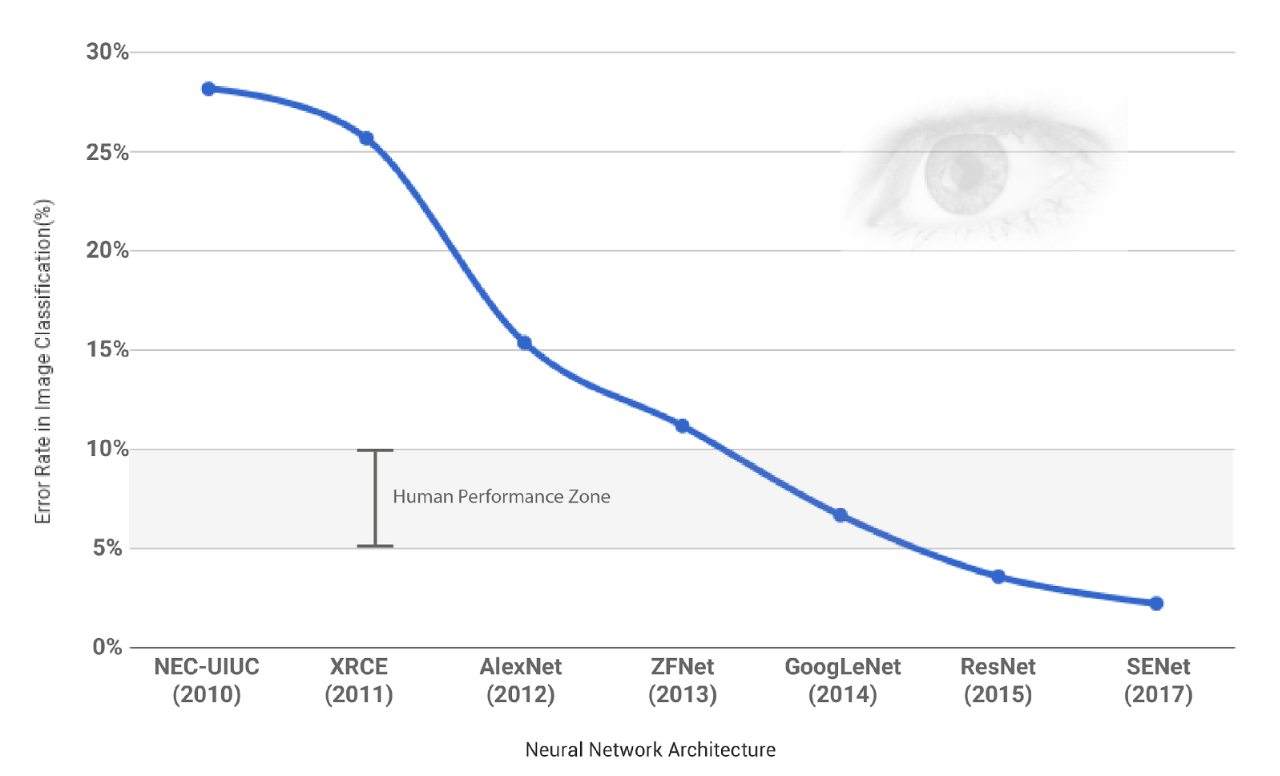
\includegraphics[width=7cm]{FIGURE13-1}
            \end{center}
        \caption{{\href{https://read01.com/zh-tw/0kxzNk.html.W6D_hegzaUk}{\url{ILSVRC\ CH Tseng}}}}
        \end{figure}
    \end{frame}
\subsection{LeNet-5 architecture}
    \begin{frame}
    \frametitle{LeNet-5 architecture: }
            \begin{figure}[H]
            \begin{center}
                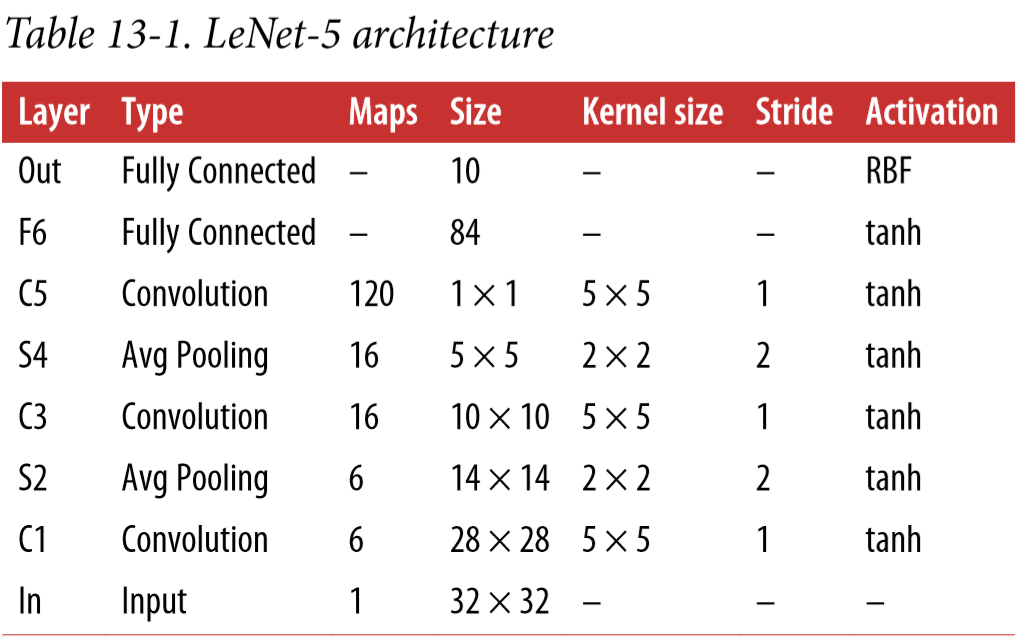
\includegraphics[width=7cm]{table13-1}
            \end{center}
        \caption{LeNet-5 architecture}
        \end{figure}
    \end{frame}
    \begin{frame}
    \frametitle{LeNet-5 architecture: }
            \begin{figure}[H]
            \begin{center}
                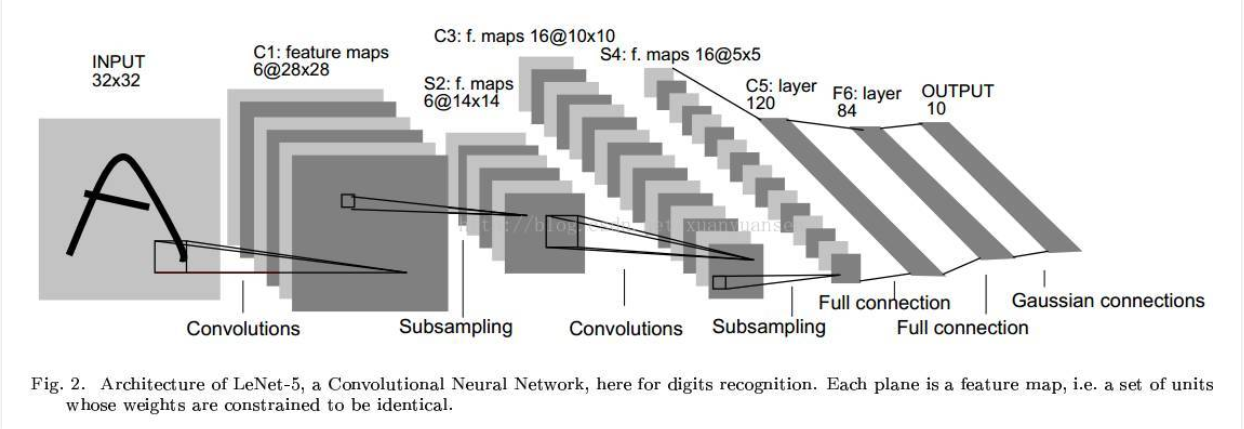
\includegraphics[width=7cm]{FIGURE13-10}
            \end{center}
        \caption{LeNet-5 architecture}
        \end{figure}
    \end{frame}
    \begin{frame}
    \frametitle{LeNet-5 architecture: }
    There are a few extra details to be noted:
        \begin{itemize}
            \item[.] MNIST images are $28 \times 28$ pixels, but they are zero-padded to $32 \times 32$ pixels and normalized before being fed to the network.
            \item[.] Most  neurons  in  C3  maps  are  connected  to  neurons  in  only  three  or  four  S2 maps (instead of all six S2 maps).
        \end{itemize}
    \end{frame}
    \begin{frame}
    \frametitle{LeNet-5 architecture: }
        \begin{figure}[H]
            \begin{center}
                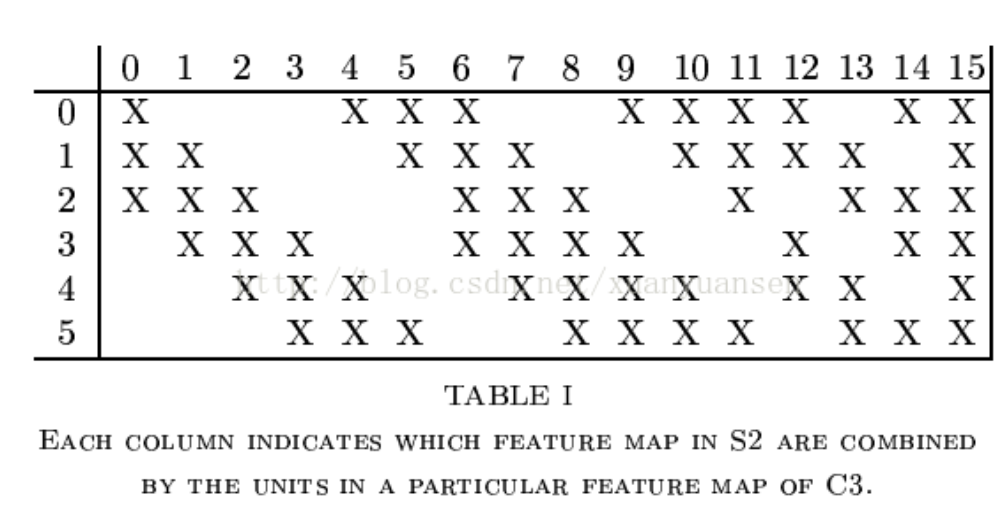
\includegraphics[width=7cm]{table13-4}
            \end{center}
        \caption{LeNet-5 architecture}
        \end{figure}
    \end{frame}
\subsection{AlexNet architectures}
    \begin{frame}
        \begin{itemize}
            \item[.] The AlexNet CNN architecture $9$ won the $2012$ ImageNet ILSVRC challenge by a large margin: it achieved $0.17$ top-$5$ error rate while the second best achieved only 26%!
            \item[.] It is quite similar to LeNet-$5$, only much larger and deeper, and it was the first to \textbf{stack convolutional layers directly on top of each other}, instead of stacking a pooling layer on top of each convolutional layer.
        \end{itemize}
    \end{frame}
    \begin{frame}
    \frametitle{AlexNet architectures: }
        \begin{figure}[H]
            \begin{center}
                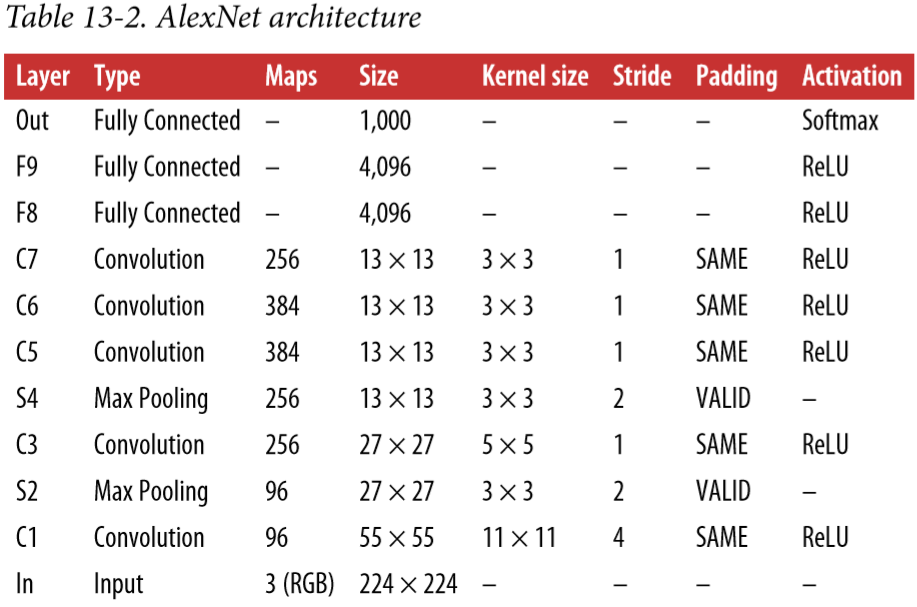
\includegraphics[width=7cm]{table13-2}
            \end{center}
        \caption{AlexNet architectures}
        \end{figure}
    \end{frame}

    \begin{frame}
    \textbf{To reduce overfitting}, the authors used two regularization techniques we discussed in previous chapters:
        \begin{itemize}
            \item[.] They applied \textbf{dropout} during training to the outputs of layers F8 and F9.
            \item[.] They performed \textbf{data augmentation} by randomly shifting the training images by various offsets, flipping them horizontally,and changing the lighting conditions.
         \end{itemize}
    \end{frame}

    \begin{frame}
    AlexNet also uses a competitive normalization step immediately after the ReLU step of layers C1 and C3, called \textbf{local response normalization}.
        Equation 13-2.(Local response normalization):
        \begin{equation}
             b_i=a_i\left(k+\alpha\sum_{j=j_{low}}^{j_{high}}\alpha_j^2\right)^{-\beta}\quad with
             \left\{\begin{array}{lr}
                 j_{high}=min\left(i+\frac{r}{2},f_n-1\right)\\
                 j_{low}=max\left(0,i-\frac{r}{2}\right)
             \end{array}
            \right.
        \end{equation}
    \end{frame}

    \begin{frame}
    \frametitle{AlexNet architectures: }
        \begin{figure}[H]
            \begin{center}
                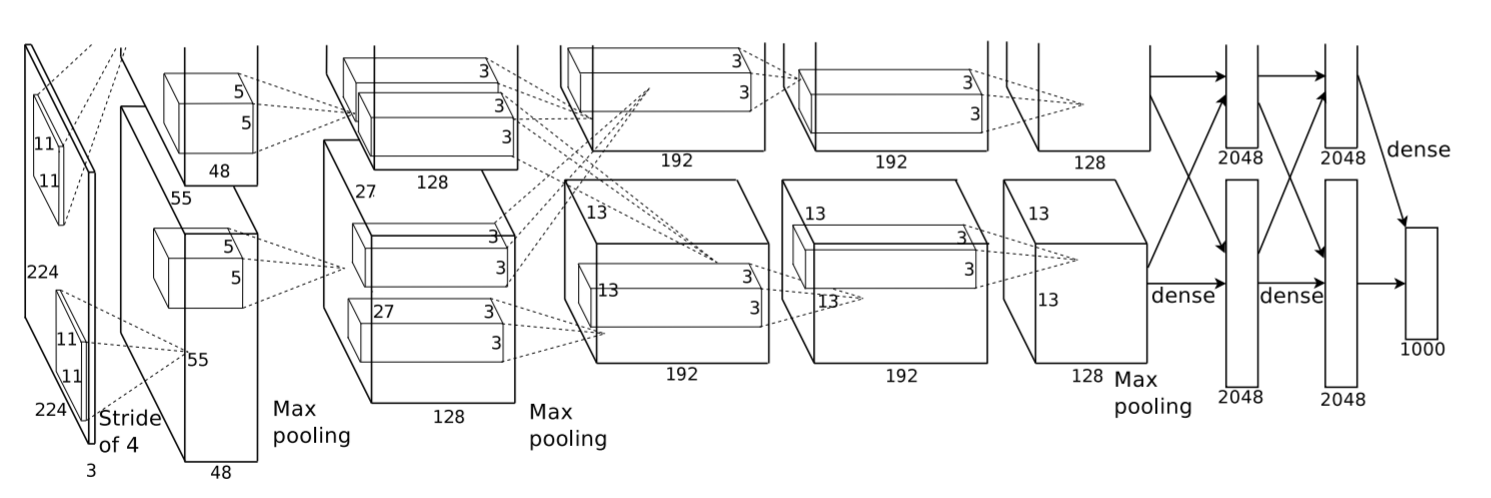
\includegraphics[width=7cm]{FIGURE13-2.png}
            \end{center}
        \caption{AlexNet architectures}
        \end{figure}
    \end{frame}
\subsection{GoogLeNet architectures}
    \begin{frame}
    \frametitle{GoogLeNet architectures: }
         \begin{figure}[H]
            \begin{center}
                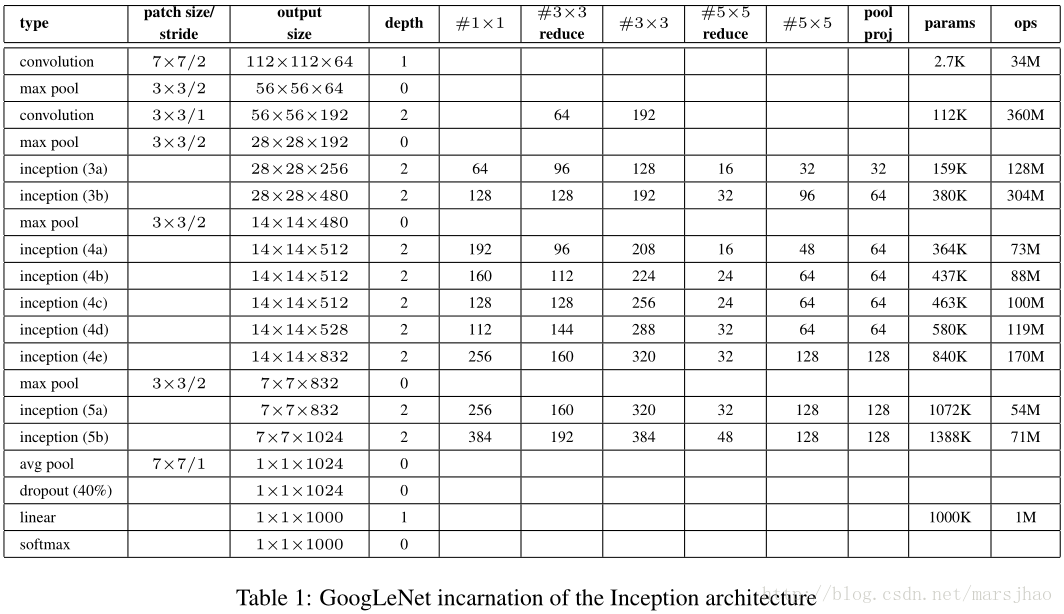
\includegraphics[width=7cm]{table13-3}
            \end{center}
        \caption{GoogLeNet architectures}
        \end{figure}
    \end{frame}

    \begin{frame}
    \frametitle{GoogLeNet architectures: }
         \begin{figure}[H]
            \begin{center}
                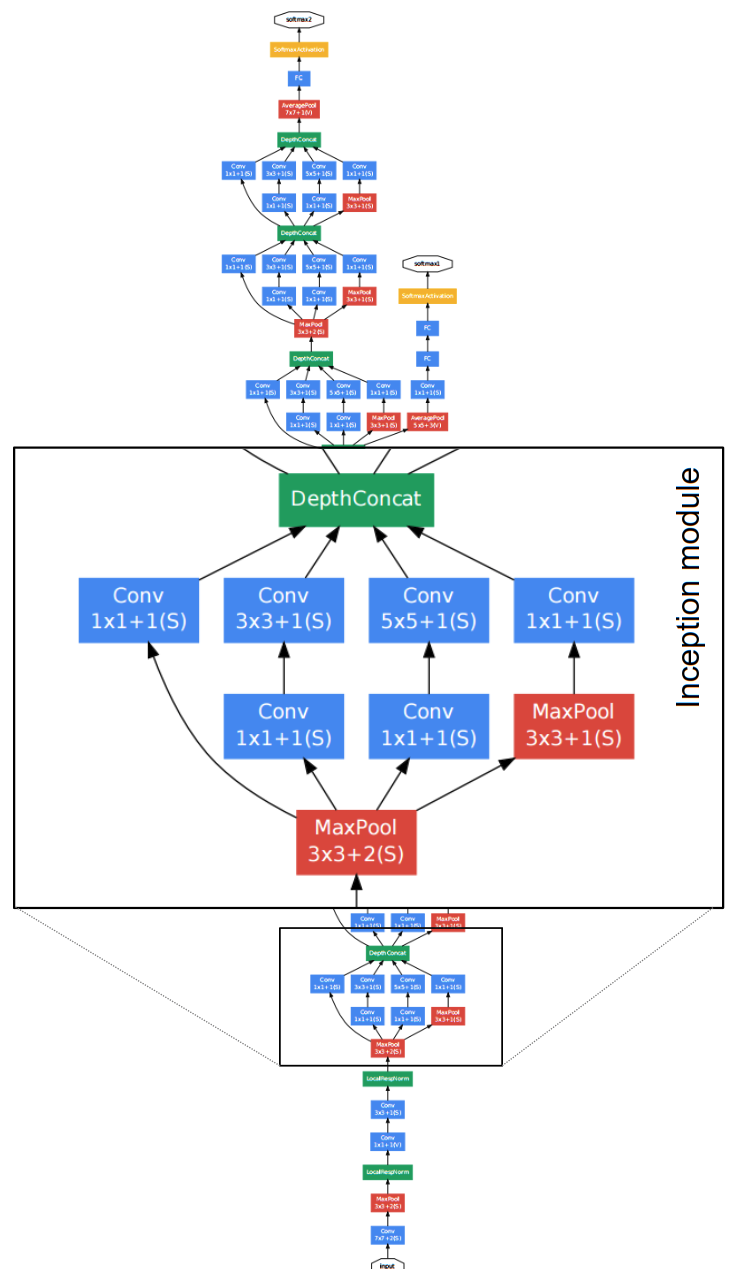
\includegraphics[width=3cm]{FIGURE13-3.png}
            \end{center}
        \caption{GoogLeNet architectures}
        \end{figure}
    \end{frame}
    \begin{frame}
    \frametitle{GoogLeNet architectures: }
         \begin{figure}[H]
            \begin{center}
                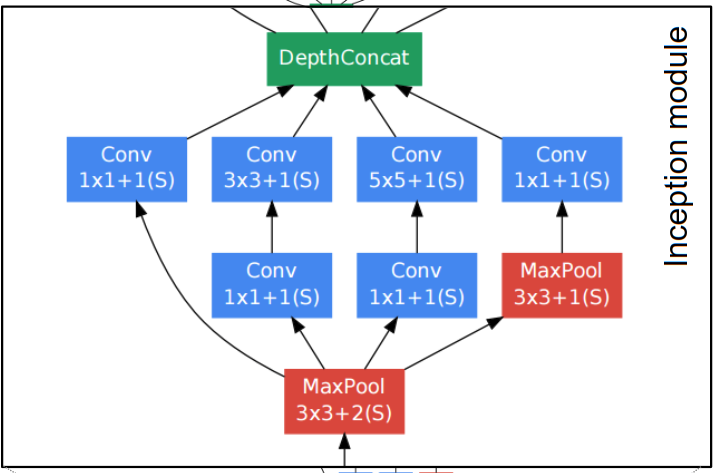
\includegraphics[width=3cm]{FIGURE13-11.png}
            \end{center}
        \caption{GoogLeNet architectures}
        \end{figure}
    \end{frame}

\subsection{ResNet architectures}
    \begin{frame}
    \frametitle{ResNet architectures: }
    \par
     the winner of the ILSVRC 2015 challenge was the Residual Network(or ResNet), developed by Kaiming He et al., which delivered an astounding top-5 error rate under 0.036
     \par
      The key to being able to train such a deep network is to use \textbf{skip connections} (also called \textbf{shortcut connections}): the signal feeding into a layer is also added to the output of a layer located a bit higher up the stack. Let’s see why this is useful.
    \end{frame}
        \begin{frame}
    \frametitle{ResNet architectures: }
         \begin{figure}[H]
            \begin{center}
                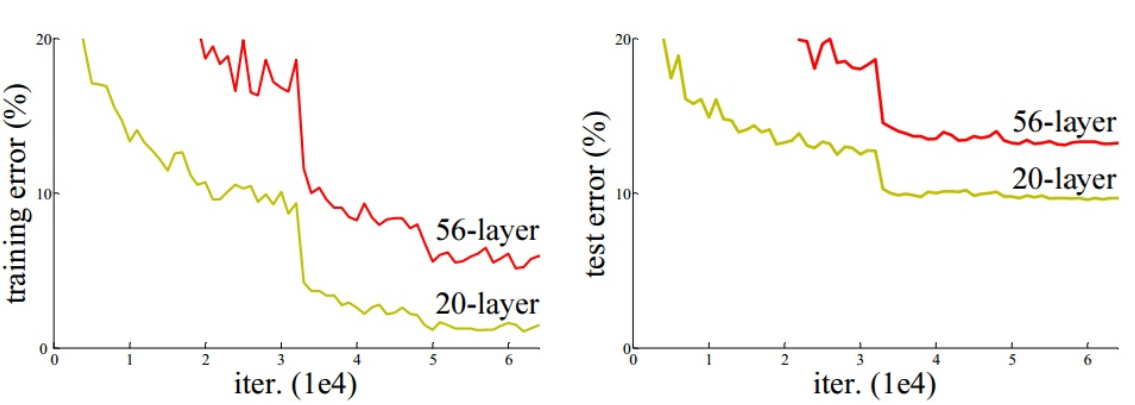
\includegraphics[width=7cm]{FIGURE13-12.png}
            \end{center}
        \caption{ResNet architectures}
        \end{figure}
    \end{frame}
    \begin{frame}
    \frametitle{ResNet architectures: }
         \begin{figure}[H]
            \begin{center}
                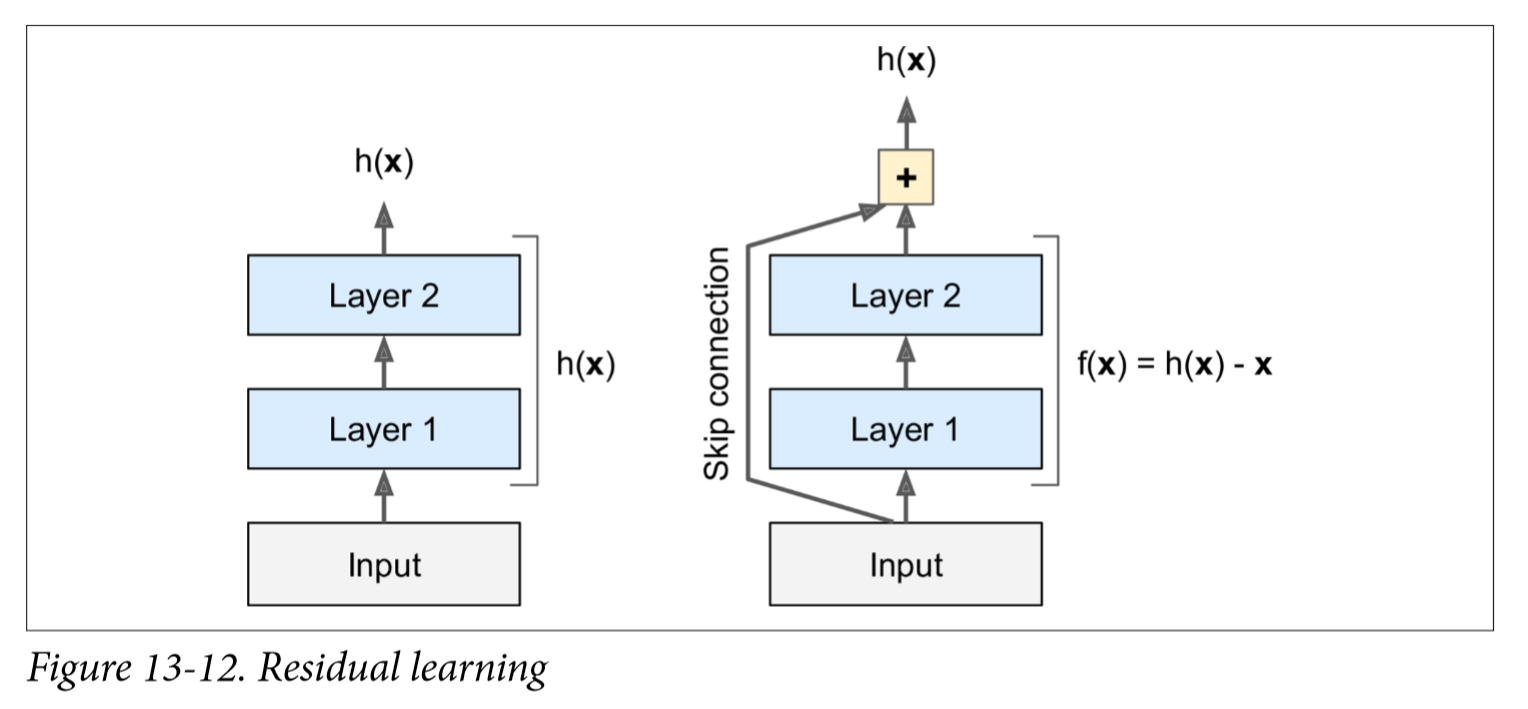
\includegraphics[width=7cm]{FIGURE13-4.png}
            \end{center}
        \caption{ResNet architectures}
        \end{figure}
    \end{frame}

    \begin{frame}
    \frametitle{ResNet architectures: }
         \begin{figure}[H]
            \begin{center}
                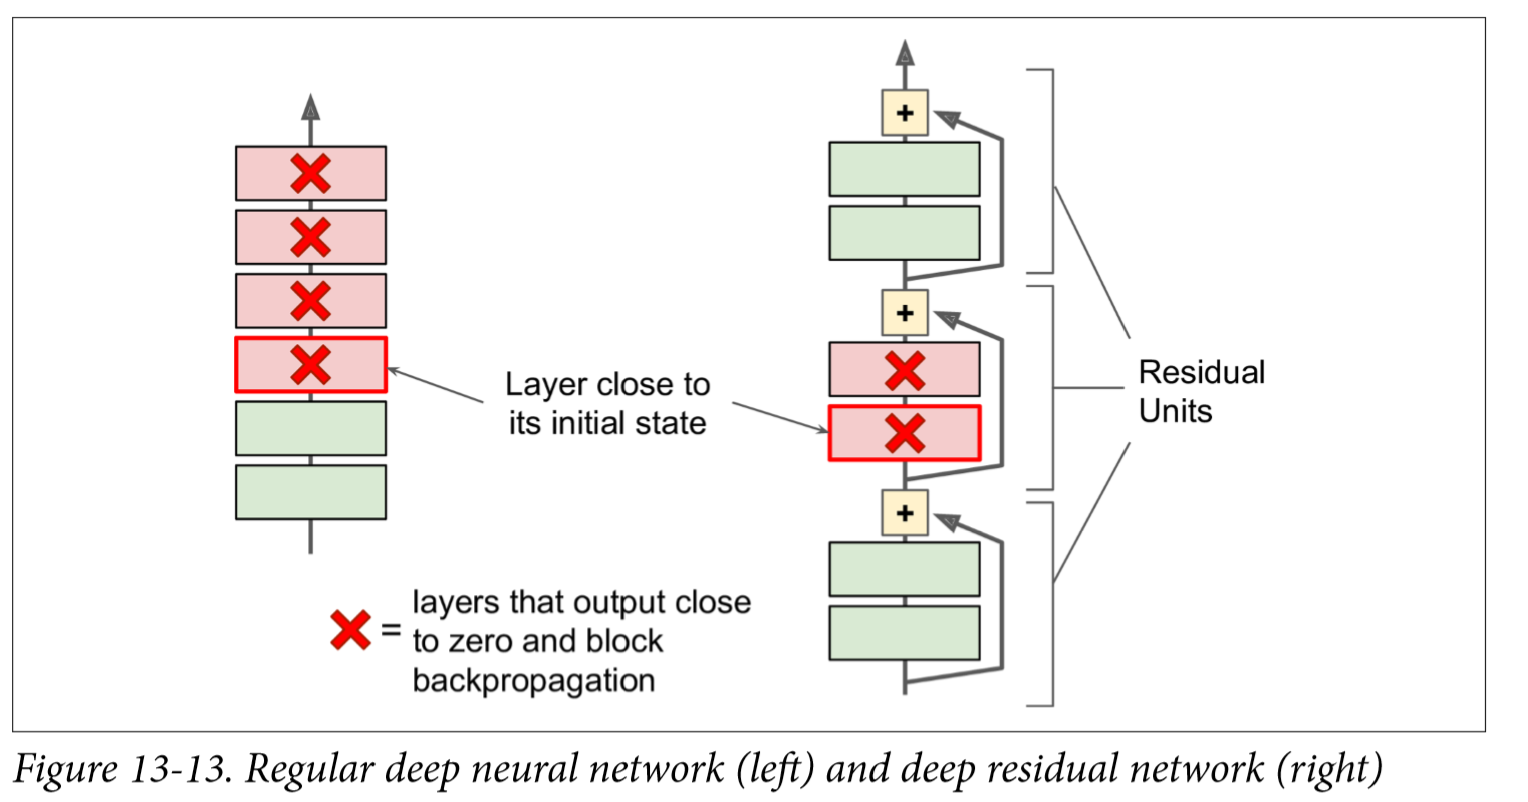
\includegraphics[width=7cm]{FIGURE13-5.png}
            \end{center}
        \caption{ResNet architectures}
        \end{figure}
    \end{frame}

    \begin{frame}
    \frametitle{ResNet architectures: }
         \begin{figure}[H]
            \begin{center}
                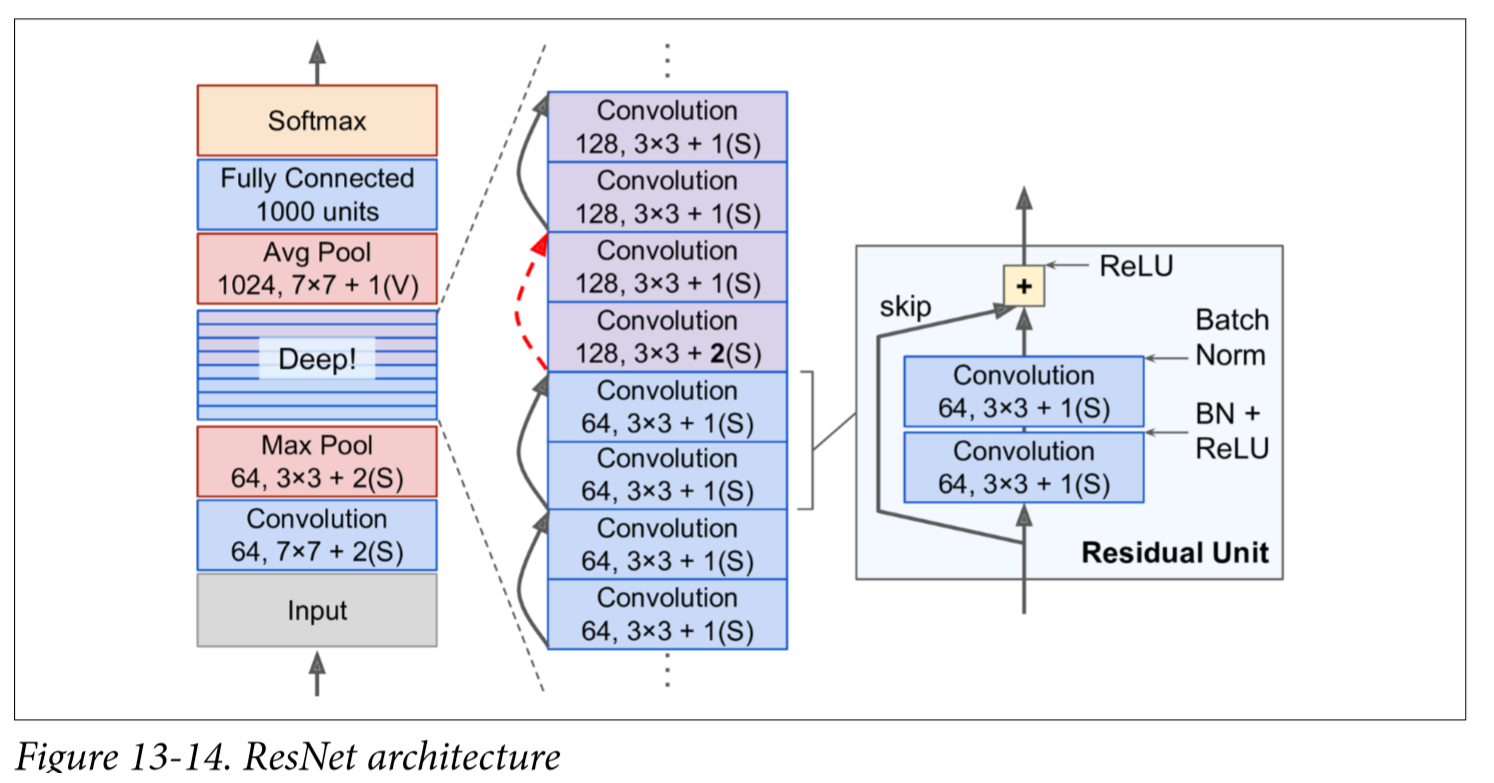
\includegraphics[width=7.5cm]{FIGURE13-6.png}
            \end{center}
        \caption{ResNet architectures}
        \end{figure}
    \end{frame}
    \begin{frame}
        \center{\huge{Thanks for listening}}
    \end{frame}
\end{document}        